\documentclass{article}
\usepackage{hyperref}
\usepackage{listings}
\usepackage{color}
\usepackage{xcolor}
\usepackage{geometry}
\usepackage{graphicx}
\usepackage{amsmath}
\usepackage{caption}
\usepackage{subcaption}
\geometry{margin=1in}
\pdfminorversion=6

\newcommand\TODO[1]{\textcolor{red}{TODO: #1}}

\newcommand\header[2]{
    \begin{center}
        {\large
        UCSD CSE 168 Assignment #1: \\
        \vspace{0.3cm}
        \Large
        #2}
    \end{center}
}

\definecolor{dkgreen}{rgb}{0,0.6,0}
\definecolor{gray}{rgb}{0.5,0.5,0.5}
\definecolor{mauve}{rgb}{0.58,0,0.82}
\lstset{frame=tb,
        aboveskip=3mm,
        belowskip=3mm,
        showstringspaces=false,
        columns=flexible,
        basicstyle={\small\ttfamily},
        numbers=none,
        numberstyle=\tiny\color{gray},
        keywordstyle=\color{blue},
        commentstyle=\color{dkgreen},
        stringstyle=\color{mauve},
        breaklines=true,
        breakatwhitespace=true,
        tabsize=2
}

\hypersetup{colorlinks=true}

\usepackage{xcolor}

\begin{document}

\header{3}{Textures, shading normals, Fresnel, and area lights}

\begin{figure}[ht]
    \centering
    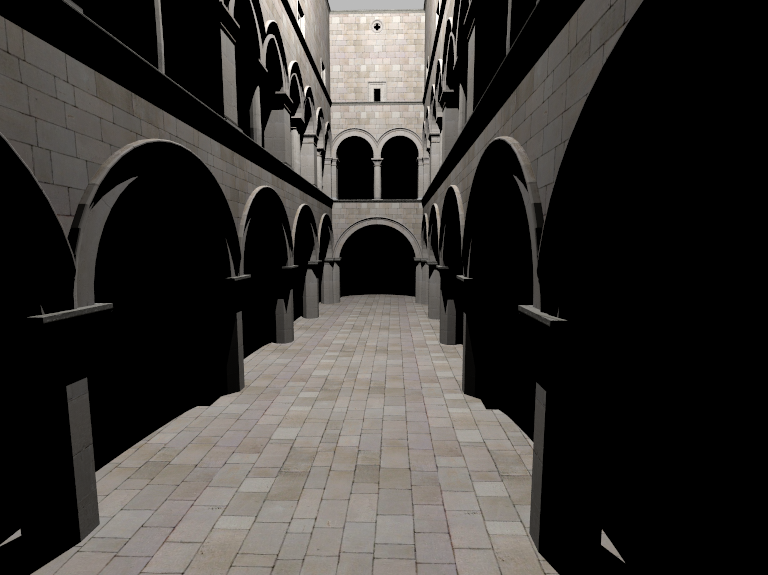
\includegraphics[width=0.2\linewidth]{imgs/hw_3_1d.png}
    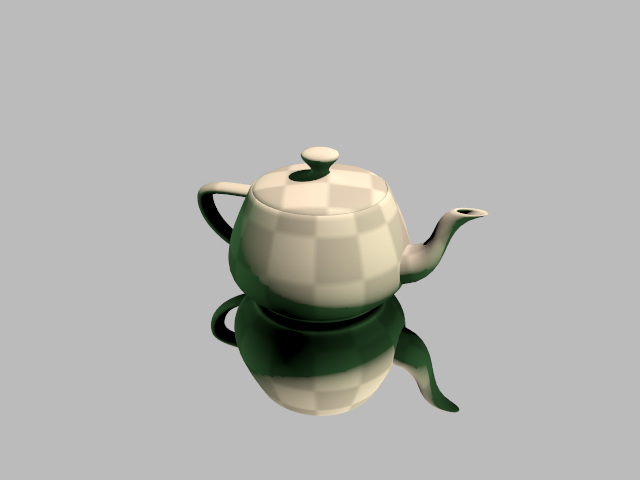
\includegraphics[width=0.2\linewidth]{imgs/hw_3_2a.png}
    \includegraphics[width=0.2\linewidth]{imgs/hw_3_3c.png}
    \includegraphics[width=0.15\linewidth]{imgs/hw_3_4a.png}
    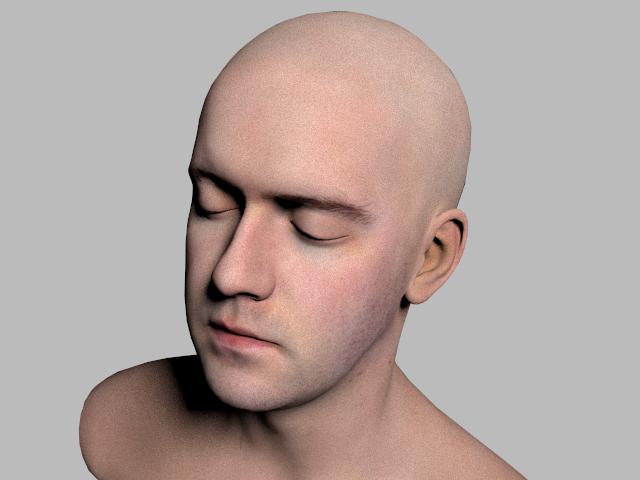
\includegraphics[width=0.2\linewidth]{imgs/hw_3_4b.png}
    \caption{Images we will render in this homework.}
    \label{fig:teaser}
\end{figure}

In the previous homework, we mostly focused on increasing the \emph{geometric complexity} of our renderer and scenes. In this homework, we're going to implement a bunch of small features for our renderer to increase the \emph{material} and \emph{lighting complexity} of our scenes (Figure~\ref{fig:teaser}). We will use both the \href{https://raytracing.github.io/books/RayTracingTheNextWeek.html}{Ray Tracing - The Next Week (RTNW)} book and the last book of the RTOW series, \href{https://raytracing.github.io/books/RayTracingTheRestOfYourLife.html}{Ray Tracing - The Rest of Your Life (RTRYL)}, for this homework.

\section{Textures (22.5 pts)}
So far, we assume constant color per object. This is kind of boring and real world objects are {\color{red}c}{\color{orange}o}{\color{green}l}{\color{blue}o}{\color{cyan}r}f{\color{magenta}u}{\color{violet}l}. The way computer graphics deal with colors on objects is through \href{https://en.wikipedia.org/wiki/Texture_mapping}{textures} (invented by Edwin Catmull in the 70s!): basically we wrap an image around a surface and define color on that image. There are two common ways to specify a texture: you can specify it \emph{procedurally} through a program, or you can use a raster image to represent the texture. We will implement the raster image texture, and the procedural texture will be bonus.

Go read \href{https://raytracing.github.io/books/RayTracingTheNextWeek.html#solidtextures}{Chapter 4} and \href{https://raytracing.github.io/books/RayTracingTheNextWeek.html#imagetexturemapping}{Chapter 6} of RTNW.

For the UV coordinates, we will use the same as the RTNW book for spheres. For triangles, there are two possiblities. First, the triangle mesh can come with its own UV coordinates per triangle vertex. You can access it through \lstinline{ParsedTriangleMesh::uvs} -- if the mesh contains UV coordinates, \lstinline{uvs} would be an array with the same size as \lstinline{positions}. To get the UV coordinates at each point, we interpolate from the three UV values from the vertices using the barycentric coordinates $(b_1, b_2)$: $u = (1 - b_1 - b_2)u_0 + b_1 * u_1 + b_2 * u_2$.
Second, if the triangle mesh does not come with UV coordinates (\lstinline{uvs.size() == 0}), we will just use the barycentric coordinates $(b_1, b_2)$ as our UV.

When looking up the texture given a UV coordinate, we will do something different from the RTNW book. Firstly, the RTNW book \emph{clamps} the UV coordinates when they are smaller than 0 or larger than 1. This is not ideal when we want to tile the textures and repeat them across the surface. Instead, we will wrap the UV coordinates around by taking a \lstinline{modulo} by one. For example, if $u = 1.5$, instead of clamping it to $1$, we wrap it to $0.5$. You may find the \lstinline{modulo} function defined in \lstinline{torrey.h} to be useful. Secondly, we introduce the parameters \lstinline{uscale, vscale, uoffset} and \lstinline{voffset} to scale and offset the UV coordinates (you can find them in \lstinline{ParsedImageTexture}). In particular, to map UV to integer image coordinates XY, we do the following:
\begin{lstlisting}[language=C++]
x = img.width * modulo(uscale * u + uoffset, 1);
y = img.height * modulo(vscale * v + uoffset, 1);
\end{lstlisting}
Finally, RTNW applies \emph{nearest neighbor} lookup. This gives blocky artifacts when zooming into a texture. Instead, we will apply \emph{bilinear} interpolation. Read the \href{https://en.wikipedia.org/wiki/Bilinear_interpolation}{Wikipedia page} for how to do it.

For loading an image, you can use the \lstinline{imread3} function defined in \lstinline{image.h}.

As usual, go to the function \lstinline{hw_3_1} in \lstinline{hw3.cpp}. Extend your previous renderer in Homework 2.5 to render images with textures. Replace the constant colors in our shading with the color provided by the textures.

In the Mitsuba scenes, the texture can be specified in two ways: they can be declared outside of the \lstinline{bsdf} and referenced in the reflectance, or they can be specified inside the bsdf.
\begin{lstlisting}[language=C++]
    <texture type="bitmap" id="grid">
        <string name="filename" value="grid.exr"/>
        <float name="uscale" value="4"/>
        <float name="vscale" value="4"/>
        <float name="uoffset" value="0.2"/>
        <float name="voffset" value="0.3"/>
    </texture>

    <bsdf type="diffuse" id="grid_material">
        <ref name="reflectance" id="grid"/>
    </bsdf>


    <bsdf type="diffuse" id="face">
        <texture name="reflectance" type="bitmap">
            <string name="filename" value="lambertian.jpg"/>
        </texture>
    </bsdf>
\end{lstlisting}

To see your results, type the following in the terminal (assuming you are in the \lstinline{torrey/build} directory):
\begin{lstlisting}[language=C++]
./torrey -hw 3_1 ../scenes/texture_test/texture.xml
./torrey -hw 3_1 ../scenes/texture_test/texture_scaled.xml
./torrey -hw 3_1 ../scenes/teapot/teapot_textured.xml
./torrey -hw 3_1 ../scenes/sponza/sponza.xml
./torrey -hw 3_1 ../scenes/head/head.xml
\end{lstlisting}
We provide the references in Figure~\ref{fig:hw_3_1}.

\begin{figure}[ht]
    \centering
    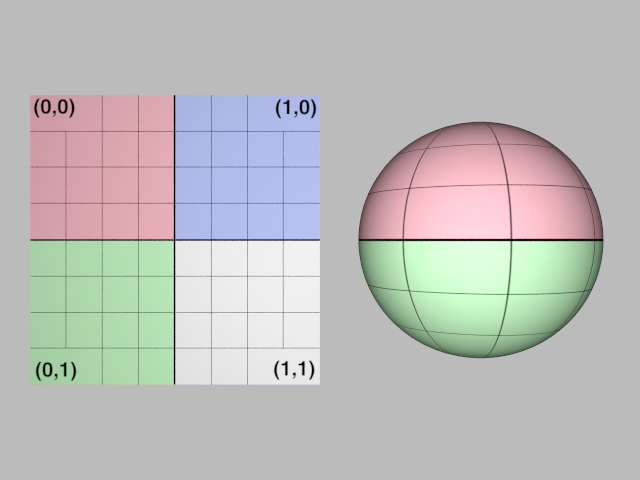
\includegraphics[width=0.19\linewidth]{imgs/hw_3_1a.png}
    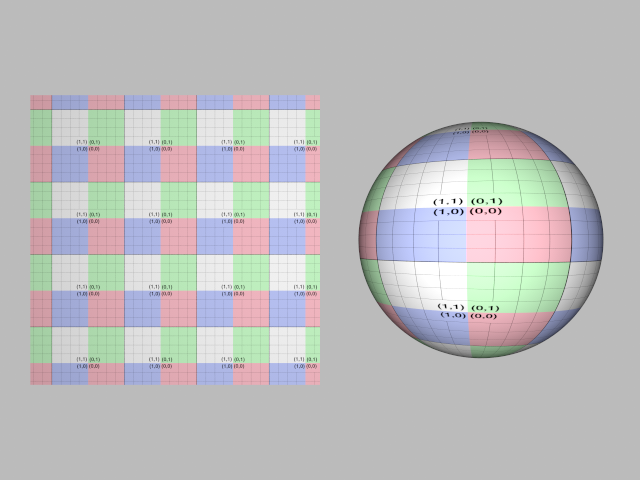
\includegraphics[width=0.19\linewidth]{imgs/hw_3_1b.png}
    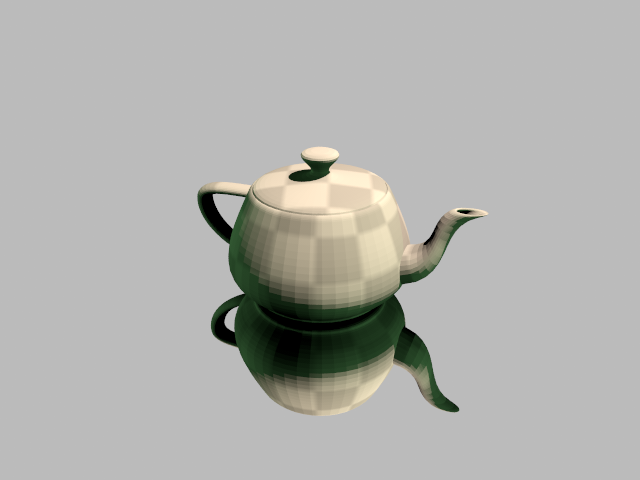
\includegraphics[width=0.19\linewidth]{imgs/hw_3_1c.png}
    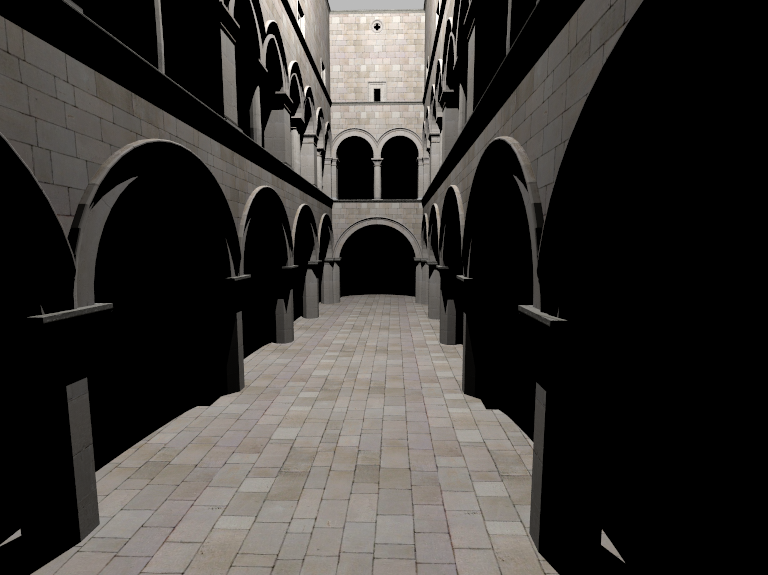
\includegraphics[width=0.19\linewidth]{imgs/hw_3_1d.png}
    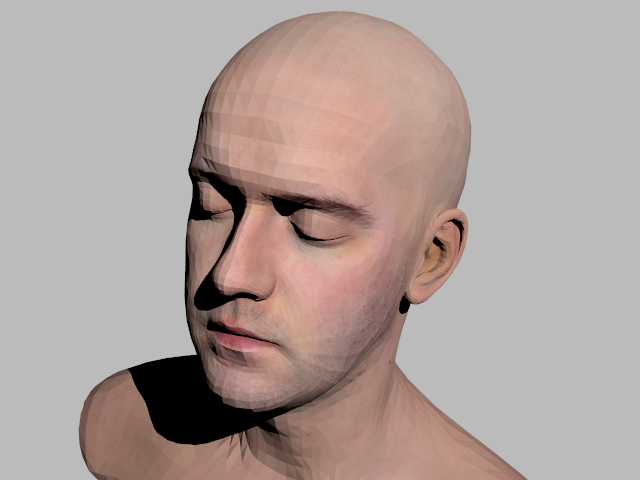
\includegraphics[width=0.19\linewidth]{imgs/hw_3_1e.png}
    \caption{Reference images for Homework 3.1.}
    \label{fig:hw_3_1}
\end{figure}

\section{Shading normals (22.5 pts)}
You have probably noticed that some of the 3D models we rendered look ``polygonal'', while we ideally want them to be smooth. One way to improve this is to increase the polygon count, but this approach seems expensive. \href{https://en.wikipedia.org/wiki/Phong_shading}{Phong} has come up with a genius way to make polygonal surfaces look smooth. The idea is to define a \emph{shading normal} per triangle vertex, and interpolate the normal within the triangle to have smooth normals. We will implement shading normals in this part.

Our \lstinline{ParsedTriangleMesh} can come with a field \lstinline{normals} which is its shading normals defined per-vertex (if \lstinline{ParsedTriangleMesh::normals.size() == 0}, then the mesh does not have shading normals). Once you hit a triangle, if it has a shading normal, interpolate the normals using the barycentric coordinates (just like how you interpolate the UV coordinates, but remember to \lstinline{normalize} after interpolation). Then, during shading, replace the normal you used with the interpolated shading normal.

As usual, type the following in the terminal to see your results:
\begin{lstlisting}[language=C++]
./torrey -hw 3_2 ../scenes/teapot/teapot_textured.xml
./torrey -hw 3_2 ../scenes/head/head.xml
\end{lstlisting}
You should render images like the ones in Figure~\ref{fig:hw_3_2}.

\begin{figure}[ht]
    \centering
    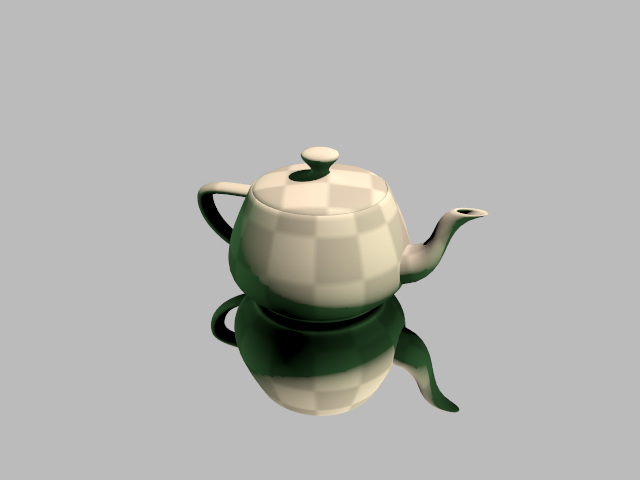
\includegraphics[width=0.3\linewidth]{imgs/hw_3_2a.png}
    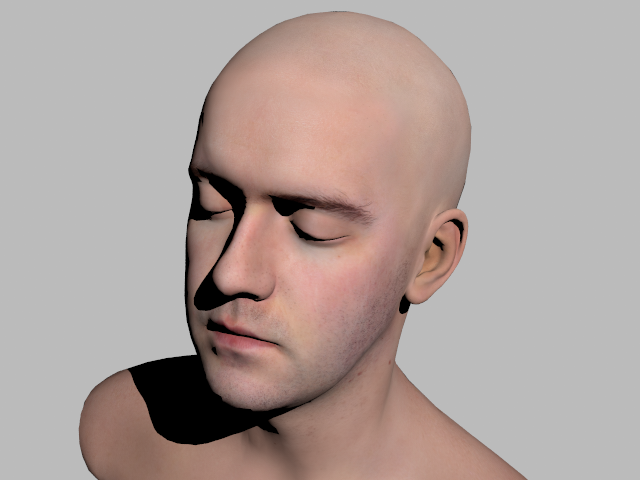
\includegraphics[width=0.3\linewidth]{imgs/hw_3_2b.png}
    \caption{Reference images for Homework 3.2.}
    \label{fig:hw_3_2}
\end{figure}

\paragraph{Quiz (5 pts):} Why does the shadow boundary for the teapot still look jaggy? Propose a way to fix it. (Hint: you may want to read Hanika's article on \href{https://jo.dreggn.org/home/2021_terminator.pdf}{Hacking the shadow terminator}.)

\section{Fresnel reflection (22.5 pts)}
Real world metals and mirrors do not reflect light equally at all angles. A prominent effect is predicted by a French physicst \href{https://en.wikipedia.org/wiki/Augustin-Jean_Fresnel}{Fresnel} using the wave theory of light. For example, metals become more white when you look at it from a \emph{grazing angle}. Many materials also get more mirror-like when we look at them from grazing angles.

In graphics, we use an approximation proposed by \href{https://en.wikipedia.org/wiki/Schlick%27s_approximation}{Christophe Schlick}:
\begin{equation}
F = F_0 + (1 - F_0) \left(1 - n \cdot l\right)^5,
\label{eq:fresnel}
\end{equation}
where $n$ is the normal and $l$ is the unit direction towards the light source. $F_0$ is the reflection when light comes in perpendicularly to the surface. For glasses and dielectric materials, $F_0$ can be well approximated by the index of refraction ($F_0 = \left(\frac{\eta_i - \eta_o}{\eta_i + \eta_o}\right)^2$ where $\eta_i$ and $\eta_o$ are the index of refraction of the two sides of the surfaces). For metals or \emph{conductors}, the actual Fresnel equation requires the index of refraction number to be described using complex numbers, and the index of refraction differs a lot depends on the wavelength of light.\footnote{\href{https://www.feynmanlectures.caltech.edu/I_31.html}{Feynman's lectures of physics} has some good introduction to this, but you might need to start reading from earlier chapters to understand the chapter I linked.} Manipulating the complex number index of refraction is not intuitive, and we do not have textured data for them either. Therefore, a common solution that gives intuitive control to metal Fresnel is to directly specify $F_0$ in RGB.\footnote{I highly recommend watching \href{https://www.youtube.com/watch?v=kEcDbl7eS0w}{Natty Hoffman's presentation} on the topic of Fresnel equation.}

Let's first add the Fresnel term to our \lstinline{mirror} material. Instead of directly multiplying the color with the reflectance, we multiply it with the Schlick Fresnel (Equation~\eqref{eq:fresnel}). 

Let's use a scene from Homework 1 to test your result:
\begin{lstlisting}[language=bash]
./torrey -hw 3_3 ../scenes/hw1_spheres/scene1.xml
\end{lstlisting}

You should see something like Figure~\ref{fig:hw_3_3_fresnel}.

\begin{figure}[ht]
    \centering
    \includegraphics[width=0.4\linewidth]{imgs/hw_3_3a.png}
    \caption{Adding Fresnel reflection to the mirror spheres.}
    \label{fig:hw_3_3_fresnel}
\end{figure}

\paragraph{Quiz (5 pts):} Change the direction $l$ to point towards the incoming ray direction in your code -- does it make a difference? Why?

Another good use of Fresnel equation is to blend between diffuse and specular materials. The physics work like this: many materials have multiple \emph{layers}. Many materials can be modeled using two layers: a dieletric \emph{coating} on top of a diffuse layer. For example, plastic, woods, and car paint usually are like this: they have an overall diffusive appearance, but also have the shiny smooth coating on top of the surface. When a light hits the dielectric layer, $F$ amount of light will reflect, and $1 - F$ amount of light will \emph{refract} into the diffuse layer. Thus we can often blend diffuse and specular layers using the Fresnel equation:
\begin{equation}
\text{specular} + (1 - F) \text{diffuse},
\end{equation}
where the specular term already includes the Fresnel equation. Figure~\ref{fig:real_world_fresnel} shows a real photograph demonstrating this effect: when we look at the table from the grazing angle, it becomes more specular, and when we look at the table from the top, it becomes more diffusive.
\begin{figure}[ht]
    \centering
    \includegraphics[width=0.3\linewidth]{imgs/fresnel_1.jpeg}
    \includegraphics[width=0.3\linewidth]{imgs/fresnel_2.jpeg}
    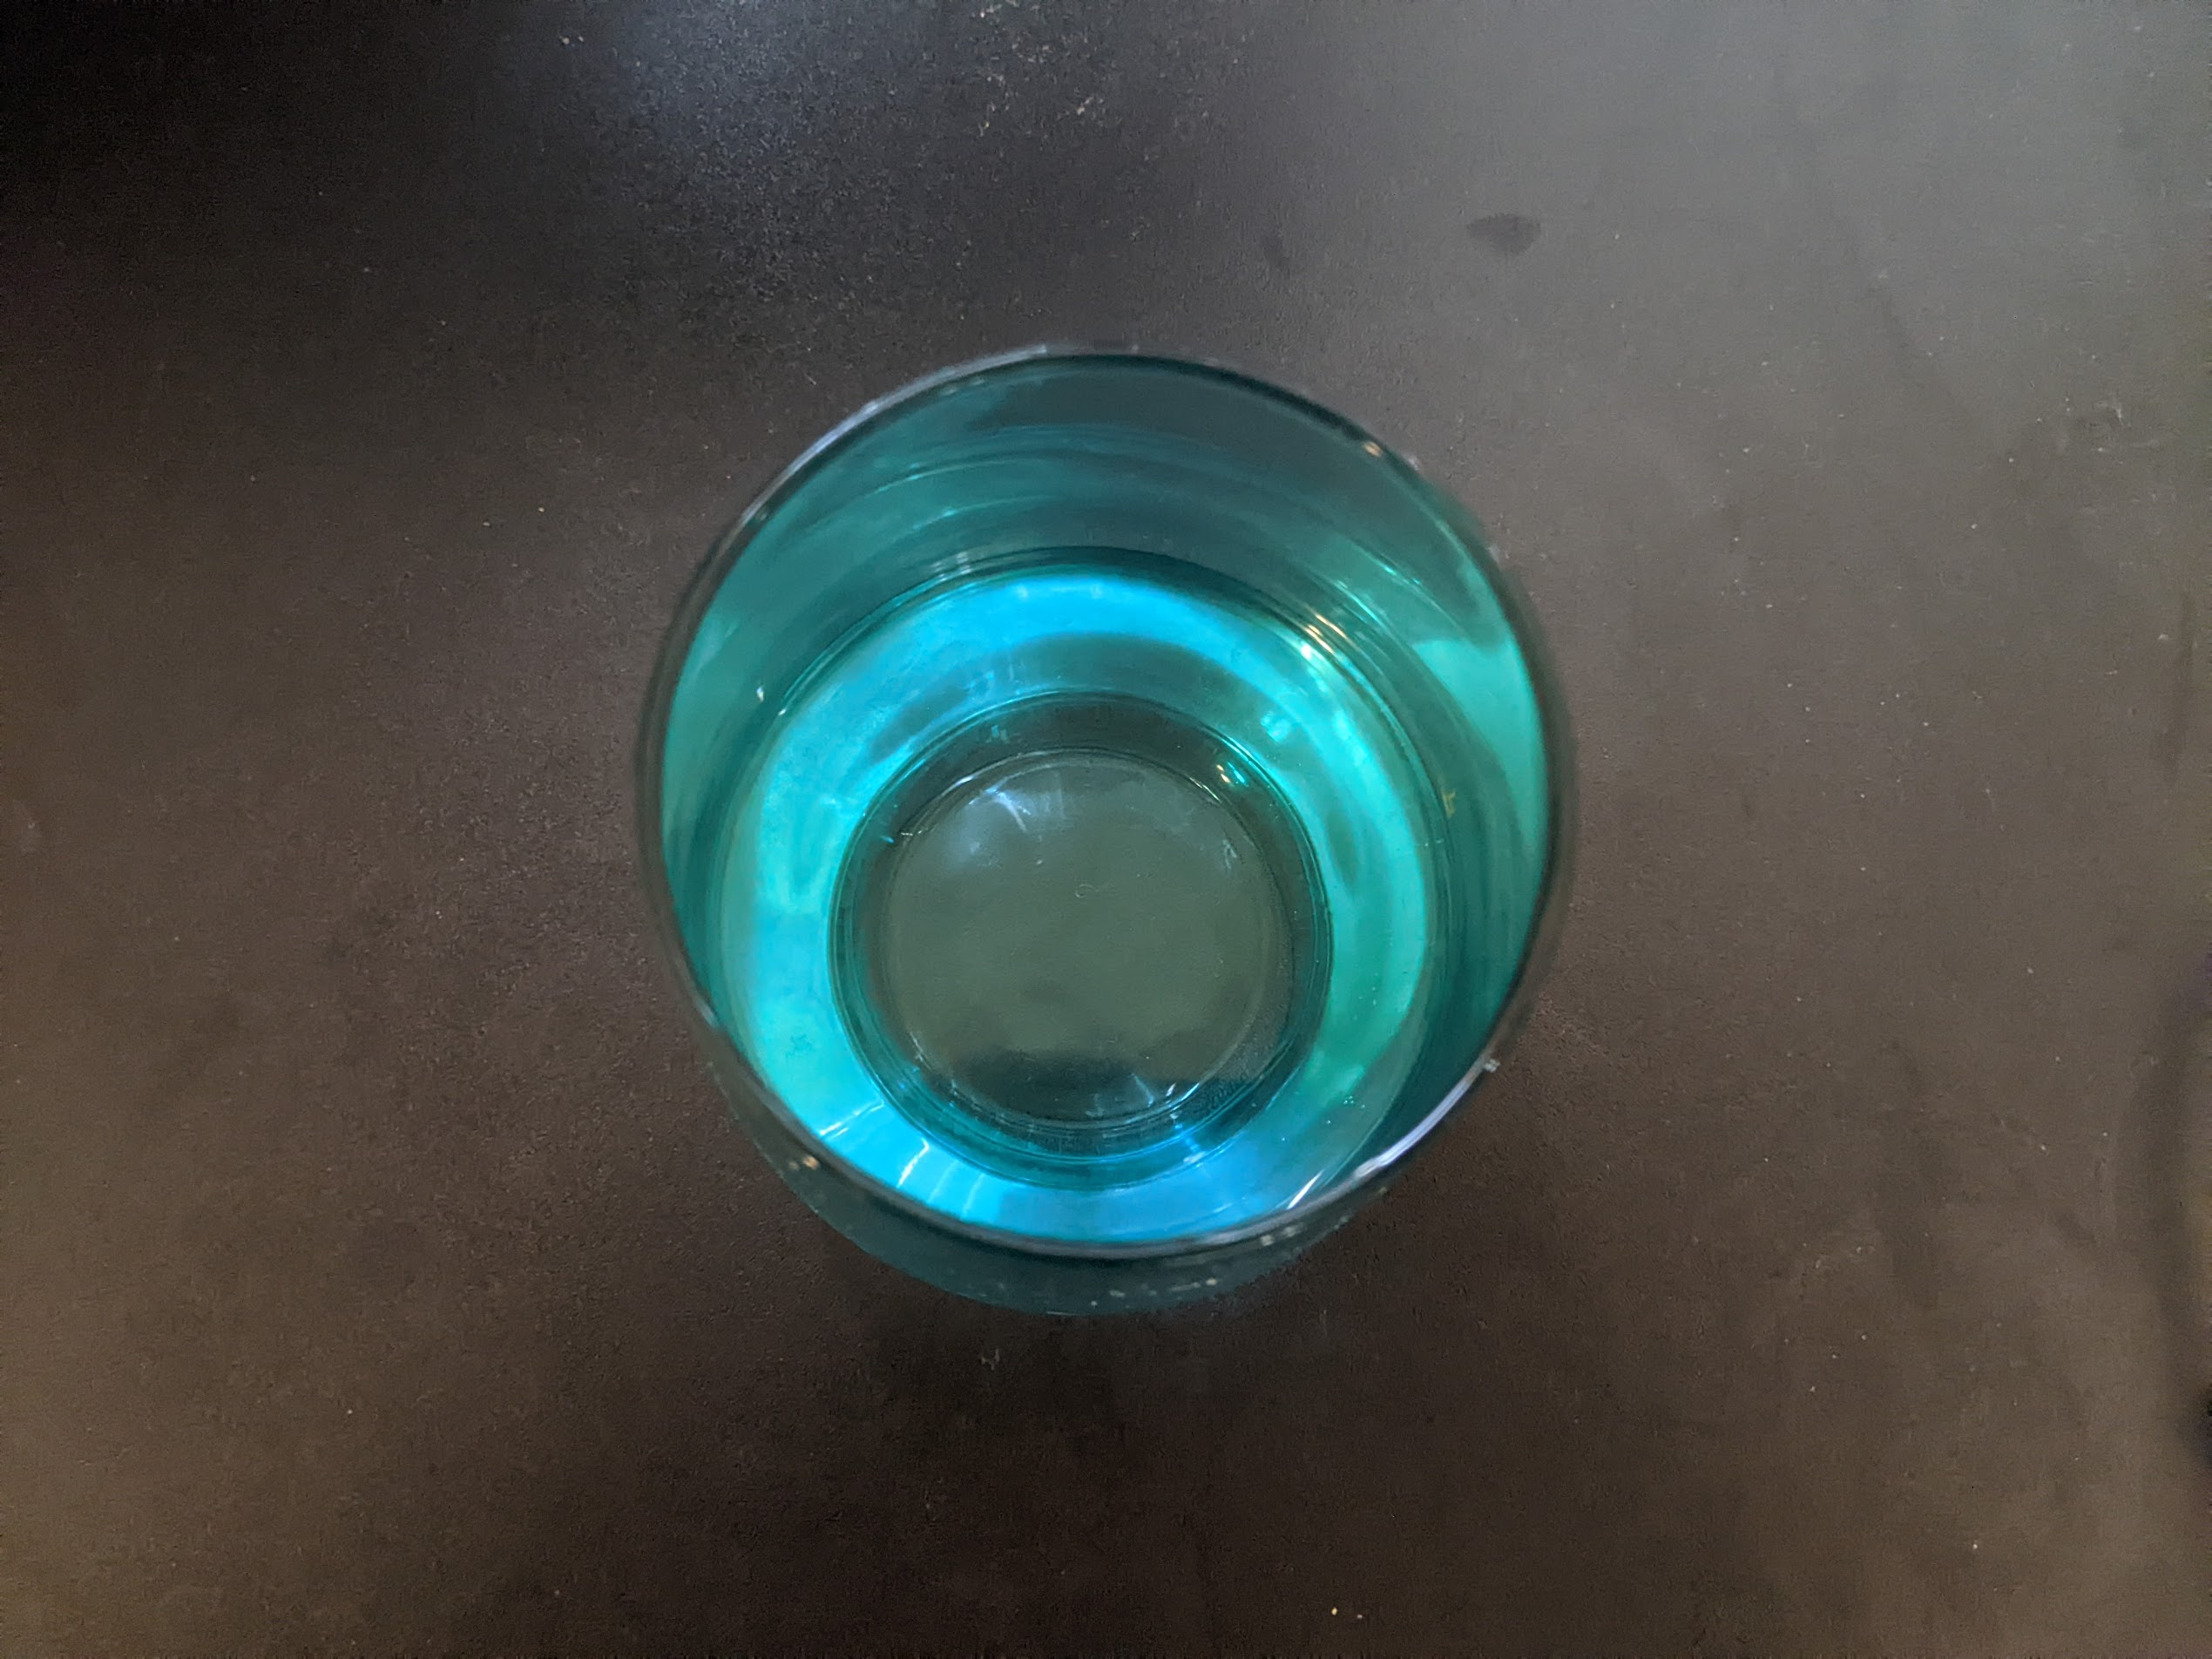
\includegraphics[width=0.3\linewidth]{imgs/fresnel_3.jpeg}
    \caption{Real world pictures showing the effect of Fresnel reflection on coated materials (look at the table).}
    \label{fig:real_world_fresnel}
\end{figure}
Since in this situation, the specular layer is usually dieletric, and these dielectric materials are usually monochromatic (i.e., the index of refraction is the same for all visible wavelength), we will use a single index of refraction parameter to control $F_0$. Assuming the index of refraction of air is $1$, we set $F_0 = \left(\frac{\eta - 1}{\eta + 1}\right)^2$ for all RGB. A common choice of $\eta$ is $1.5$.

Implement this Fresnel-based blending in the \lstinline{plastic} material (the information is stored in \lstinline{ParsedPlastic} in the scene). Use the following scenes to test your method:
\begin{lstlisting}[language=bash]
./torrey -hw 3_3 ../scenes/bunny/bunny_plastic_floor_view_low.xml
./torrey -hw 3_3 ../scenes/bunny/bunny_plastic_floor_view_mid.xml
./torrey -hw 3_3 ../scenes/bunny/bunny_plastic_floor_view_high.xml
\end{lstlisting}
You should see images like the ones in Figure~\ref{fig:bunny_fresnel}.
\begin{figure}[ht]
    \centering
    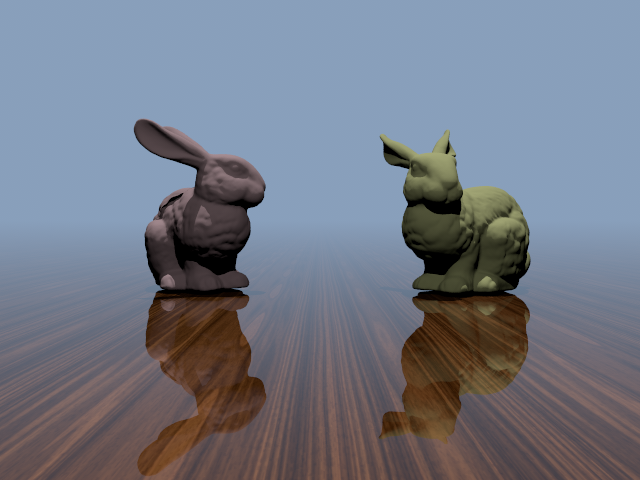
\includegraphics[width=0.3\linewidth]{imgs/hw_3_3b.png}
    \includegraphics[width=0.3\linewidth]{imgs/hw_3_3c.png}
    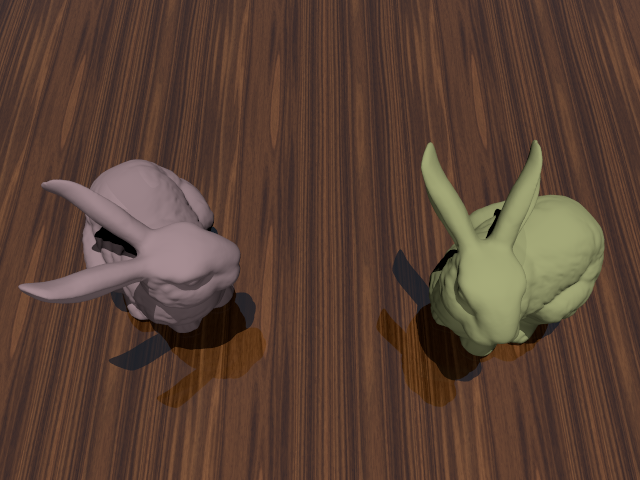
\includegraphics[width=0.3\linewidth]{imgs/hw_3_3d.png}
    \caption{Our simulation of Figure~\ref{fig:real_world_fresnel}.}
    \label{fig:bunny_fresnel}
\end{figure}

\section{Area lights (22.5 pts)}
This part is a bit more mathematically involved (the concept is very simple, but I am trying to prepare you for the more involved concepts in the later homework and in the future), but the implementation should be relatively easy.

So far all our scenes are rendered with point lights. Point lights are nice for situations where you want your shadow to have hard boundaries, but sometimes we want softer lighting. We achieve this by turning our geometric objects themselves into lights. You can think of them as an infinite collection of small point lights (but each of them only emit light towards the direction the surface is facing, instead of emitting light to all directions).

Evaluating area lights is then easy: \textbf{we randomly choose a point on the area light, and average over their contributions}! But you will see that working out what exactly do we mean by \emph{randomly choosing a point} and what exactly do we mean by \emph{contributions} can be a bit subtle. You can try to tweak the numbers until it looks right, but whatever you come up with may not work in a different scene. To make everything physically correct and consistent, we need to borrow the power of calculus -- the mathematics about infinitesimal points.

The contribution of an area light is defined by an integral over all points $x$ on the surface $S$ of a light source:
\begin{equation}
    \int_{x \in S} f(x) \mathrm{d}A(x)
    \label{eq:area_light_integral}
\end{equation}
where $\mathrm{d}A(x)$ means \emph{an infinitesimal area around x on the surface}\footnote{This notation is a bit different from the usual \emph{Riemannian integral} people learn in calculus 101. If you love math, check out \href{https://www.youtube.com/watch?v=LDNDTOVnKJk}{this video} for a cool introduction to Lesbeque integration and measure theory. You don't need to understand any of these to understand this class though.}, and $f(x)$ is similar to the contribution of a single point light located at $x$:
\begin{equation}
    f(x) = \frac{K_d \cdot \max\left(n_s \cdot l, 0\right)}{\pi} \cdot \frac{I \max\left(-n_x \cdot l, 0\right)}{d^2} \cdot \text{visibility},
    \label{eq:area_light_integrand}
\end{equation}
where $K_d$ is the diffuse reflectance, $n_s$ is the normal at the shading point, $l$ is the unit vector pointing from the shading point towards $x$, $n_x$ is the normal at point $x$ on the light source (we will use the geometric normal instead of shading normals -- we will explain why in Homework 4), and $d$ is the distance between the shading point and $x$.

\paragraph{Quiz (5 pts):} Compare Equation~\eqref{eq:area_light_integrand} to the point light contribution we introduced in Homework 1: why do we need an extra cosine term?

How do we evaluate the integral (Equation~\eqref{eq:area_light_integral})? In colleage calculus, we often attempt to derive a closed-form solution for the integral, but that is usually hard because of the visibility term and the arbitrary shape the area light can take. Thus, we approximate the integral using a discrete sum, and such approach is called Monte Carlo integration. Read \href{https://raytracing.github.io/books/RayTracingTheRestOfYourLife.html#asimplemontecarloprogram}{Chapter 2-4} of RTRYL to understand the basics of Monte Carlo integration. It is also useful to read \href{https://raytracing.github.io/books/RayTracingTheRestOfYourLife.html#samplinglightsdirectly}{Chapter 9}.

Let's be a bit more concrete. We want to sample points on the surface to do Monte Carlo integration.
We also have the ability to generate uniformly distributed random numbers between $[0, 1]$. Our goal is to connect between the uniform random numbers and the random points on the surface.
Our surface $S$ can either be a triangle or a sphere. Let's start with a sphere. In this case, given a sphere centered at $c$ with radius $r$, we can rewrite Equation~\eqref{eq:area_light_integral} in to a \href{https://en.wikipedia.org/wiki/Spherical_coordinate_system}{spherical coordinate system}:
\begin{equation}
    \int_{x \in S} f(x) \mathrm{d}A(x) = \int_{0}^{2\pi}\int_{0}^{\pi} f(x(\theta, \phi)) r^2 \sin\theta \mathrm{d}\theta \mathrm{d} \phi,
    \label{eq:area_light_spherical}
\end{equation}
where
\begin{equation}
    x(\theta, \phi) = c + r \left(\sin\theta \cos\phi, \sin\theta \sin\phi, \cos\theta \right).
\end{equation}
Here, we take the convention that $\theta$ is the elevation angle, and $\phi$ is the azimuthal angle. We need to multiply by $r^2 \sin\theta$ since it is the Jacobian determinant between the two set of integration variables.\footnote{You see, the definition of an integral is \emph{not} unique upon its integrand, it also depends on which variables you are integrating. The Jacobian captures the ratio between the infinitesimal volumes of these variables. If you love math, a more general concept is called ``Radon-Nikodym derivative''.} See the \href{https://en.wikipedia.org/wiki/Spherical_coordinate_system#Integration_and_differentiation_in_spherical_coordinates}{Wikipedia page} or \href{http://6degreesoffreedom.co/circle-random-sampling/}{this blog post} to see how this is derived.

Notice that now that we can generate uniform random numbers for $\theta$ and $\phi$ by generating two numbers between $[0, 1]$ and scale them to be between $[0, \pi]$ and $[0, 2\pi]$ respectively. This allows us to apply Monte Carlo integration:
\begin{equation}
    \int_{0}^{2\pi}\int_{0}^{\pi} f(x(\theta, \phi)) r^2 \sin\theta \mathrm{d}\theta \mathrm{d} \phi
    \approx \frac{2\pi^2 r^2}{N} \sum_i^N f(x(\theta_i, \phi_i))\sin\theta_i.
    \label{eq:naive_monte_carlo_sphere}
\end{equation}
Note that the factor $2\pi^2 r^2 \sin\theta_i$ we multiply to $f(x)$ is exactly the reciprocal of the \emph{probability density function} (PDF) of our sample $x$ (recall \href{https://raytracing.github.io/books/RayTracingTheRestOfYourLife.html#onedimensionalmcintegration/importancesampling}{Chapter 3.4} of RTRYL). Throughout this homework, we will use $N=1$.

We can do slightly better though. Notice the extra $\sin\theta$ factor in our Jacobian/PDF. This indicates that our samples do not uniformly distribute on the sphere: they have higher density when $\theta$ is close to the two polars of the sphere.

To do one step better, we can apply a \emph{change of variable} to rewrite the integral again, such that the Jacobian of the change of variable is $\frac{1}{\sin\theta_i}$. This change of variable will allow us to uniformly generate a set of points on the sphere. To achieve this, we need to apply \emph{inverse transform sampling}. 

We want to find two variables $u_1, u_2$ such that a mapping $\theta, \phi = M(u_1, u_2)$ has the Jacobian that is proportional to $\frac{1}{\sin\theta}$. Since our Jacobian does not depend on $\phi$, we can simplify the problem to finding a variable $u_1$ such that $\theta = M(u_1)$ and $M'(u_1) \propto \frac{1}{\sin\theta}$. Notice how this has become an \emph{antiderivative} problem: we want to find a function $M$ whose derivative is something specific. There is one awkward thing though: $M'(u_1)$ takes $u_1$ as input, but the derivative is specified in the output space $\theta$. The way we resolve this is to first find the inverse $M^{-1}(\theta)$. The derivative specification becomes ${M^{-1}}'(\theta) \propto \sin\theta$ (this comes from the \href{https://en.wikipedia.org/wiki/Inverse_function_theorem}{inverse function theorem}). 

Since we know that ${M^{-1}}'(\theta)$ is exactly the PDF of our sampling process, we know that it has to integrate to one:
\begin{equation}
\int_{0}^{\pi} {M^{-1}}'(\theta) \mathrm{d}\theta = C\int_{0}^{\pi} \sin\theta \mathrm{d}\theta = 1.
\end{equation}
Since $\int_{0}^{\pi} \sin\theta \mathrm{d}\theta = 2$, we have $C = \frac{1}{2}$ and ${M^{-1}}'(\theta) = \frac{\sin\theta}{2}$. To get $M^{-1}$ from its derivative, we simply integrate it:
\begin{equation}
M^{-1}(\theta) = \int_{0}^{\theta} \frac{\sin\hat{\theta}}{2} \mathrm{d}\hat{\theta} = \frac{1}{2}\left(1 - \cos\theta\right).
\end{equation}
To get $M(u_1)$ we can just invert $M^{-1}(\theta)$:
\begin{equation}
\theta = M(u_1) = \cos^{-1}\left(1 - 2u_1\right).
\end{equation}
Just to make things more unify, we can also generate $\phi$ from $u_2$:
\begin{equation}
\phi = 2\pi u_2.
\end{equation}
Thus, we have found a change of variable to rewrite Equation~\eqref{eq:naive_monte_carlo_sphere} to remove the $\sin\theta$ term:
\begin{equation}
    \int_{0}^{2\pi}\int_{0}^{\pi} f(x(\theta, \phi)) r^2 \sin\theta \mathrm{d}\theta \mathrm{d} \phi =
    \int_{0}^{1}\int_{0}^{1} f(x(M(u_1, u_2))) r^2 (2 \cdot 2\pi) \mathrm{d}u_1 \mathrm{d}u_2.
    \label{eq:uniform_monte_carlo_sphere}
\end{equation}
The extra $2 \cdot 2\pi$ factor comes from two sources: the $2$ comes from the constant $C$, and the $2\pi$ comes from the mapping between $u_2$ and $\phi$. Notice how the extra factors simplifies to $4\pi r^2$ -- the surface area of a sphere, which is the reciprocal of the PDF of a uniform distribution on it! We can then discretize the second integral in Equation~\eqref{eq:uniform_monte_carlo_sphere}.

If my explanation does not quite work for you, \href{http://6degreesoffreedom.co/circle-random-sampling/}{this blog post} explains the same thing. Make sure you are comfortable with this -- we will ask you to do it next time!

We can perform the similar process for triangles. We will omit the derivation (see \href{https://www.pbr-book.org/3ed-2018/Monte_Carlo_Integration/2D_Sampling_with_Multidimensional_Transformations#SamplingaTriangle}{PBRT} if you are interested, we also talk about it in the lectures). To uniformly sample a point on a triangle, use the following mapping:
\begin{equation}
\begin{aligned}
b_1 &= 1 - \sqrt{u_1} \\
b_2 &= u_2 \sqrt{u_1} \\
x &= (1 - b_1 - b_2) p_0 + b_1 p_1 + b_2 p_2.
\end{aligned}
\end{equation}
and the Jacobian factor is the area of the triangle.

Now, given these, implement area lights in your renderer. Area lights are represented in the \lstinline{ParsedScene} data structures in the following way: for each \lstinline{ParsedSphere} and \lstinline{ParsedTriangleMesh}, if it is an area light, then \lstinline{ParsedSphere::area_light_id} and \lstinline{ParsedTriangleMesh::area_light_id} would be a number that is larger than or equal to zero. If it is not, the ID is set to \lstinline{-1}. The area lights are also in the list of lights. They have the type \lstinline{ParsedDiffuseAreaLight} and the structure contains the ID to the shape and the color $I$ of the light.

You will need to handle two cases: 1) When a ray hits a diffuse surface, you should loop over the lights as usual, sample a point on each light, and evaluate the contribution. 2) When a ray hits an area light, you should return the color of the light directly.

Finally, for triangle lights, we do not let it emit light in the backfacing direction. We will use the shading normals to decide which direction is the front facing direction. When sampling a point on the surface, you would usually want to get its normal as well (for evaluating $n_x \cdot l$ in Equation~\eqref{eq:area_light_integrand}). Return the geometric normal for $n_x$, but flip it if it is facing a different direction than the shading normal.

\paragraph{Code structure.} I find the following (pseudo)code structure for computing the color given a ray to be cleaner. You don't have to do exactly the same as me.
\begin{lstlisting}[language=python]
def radiance(scene, ray, rng):
  if (ray intersect scene):
    # [emission] add emission of the intersected shape
    # ...
    # [direct_lighting] loop over lights, sample them, and sum over their contributions
    # ...
    # [scattering] recursively tracing the ray by calling radiance
    # ...
  else:
    return scene.background_color
\end{lstlisting}

To test your rendering, use the following commands:
\begin{lstlisting}[language=bash]
./torrey -hw 3_4 ../scenes/cbox/cbox_area_light_spheres.xml
./torrey -hw 3_4 ../scenes/head/head_spherical_light.xml
\end{lstlisting}

\paragraph{Quiz (0 pts, we won't grade it):} Compare the sampling efficiency of an implementation Equation~\eqref{eq:naive_monte_carlo_sphere} and the uniform sphere sampling.

They should render into images like the ones in Figure~\ref{fig:hw_3_4}. 

\begin{figure}[ht]
    \centering
    \includegraphics[width=0.4\linewidth]{imgs/hw_3_4a.png}
    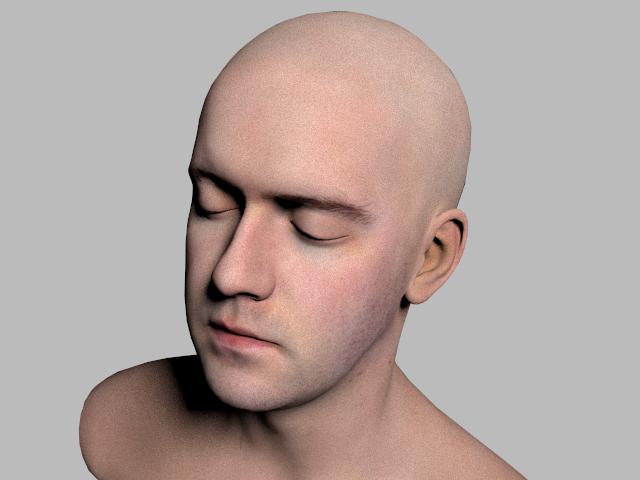
\includegraphics[width=0.4\linewidth]{imgs/hw_3_4b.png}
    \caption{Reference images for Homework 3.4.}
    \label{fig:hw_3_4}
\end{figure}

\section{Design your own scene (10 pts)}
The fun time comes again! Design your own scenes and render them. Use the features you implemented above.

\section{Bonus: Perlin noise (15 pts)}
Read \href{https://raytracing.github.io/books/RayTracingTheNextWeek.html#perlinnoise}{Chapter 5} of RTNW book and implement a procedural Perlin noise.

\section{Bonus: Volumes (15 pts)}
Read \href{https://raytracing.github.io/books/RayTracingTheNextWeek.html#volumes}{Chapter 9} of RTNW book and implement homogeneous volumes.

\section{Bonus: Schlick Fresnel vs actual Fresnel (15 pts)}
Watch \href{https://www.youtube.com/watch?v=kEcDbl7eS0w}{Natty Hoffman's presentation} on Fresnel equation and write a summary of what his points are. Write about whether you agree with him or not too.

\section{Bonus: Stratification (15 pts)}
Read \href{https://raytracing.github.io/books/RayTracingTheRestOfYourLife.html#asimplemontecarloprogram/stratifiedsamples(jittering)}{Chapter 2.3} of RTRYL and implement stratified samples for your area light sampling. Read \href{https://www.pbr-book.org/3ed-2018/Sampling_and_Reconstruction/Stratified_Sampling}{PBRT} to understand how to generalize it to higher-dimensional sampling using shuffling (the shuffling technique is introduced to graphics by \href{https://graphics.pixar.com/library/StochasticSampling/paper.pdf}{Rob Cook} and is very similar to a classical statistics technique called \href{https://en.wikipedia.org/wiki/Latin_hypercube_sampling}{Latin hypercube sampling}).

\section{Bonus: sample one light at a time (15 pts)}
Our sampling strategy currently samples one point for each light. This can be inconvienent when there is a huge amount of lights. An alternative strategy is to sample one light at a time. So you will pick a light first, then pick a point on the light. To pick a light, we want to sample based on its intensity and its surface area. You may want to read \href{https://www.pbr-book.org/3ed-2018/Monte_Carlo_Integration/Sampling_Random_Variables#x1-Example:Piecewise-Constant1DFunctions}{PBRT} for how to sample a discrete distribution. Implement this strategy and compare to your original method.

\section{Bonus: More efficient spherical light sampling (15 pts)}
Our sampling for spherical lights is not very efficient: it randomly chooses a point on a sphere, so that is 50\% of chance it will be blocked. Read \href{https://www.pbr-book.org/3ed-2018/Light_Transport_I_Surface_Reflection/Sampling_Light_Sources#x2-SamplingSpheres}{PBRT} or \href{https://raytracing.github.io/books/RayTracingTheRestOfYourLife.html#cleaninguppdfmanagement/samplingasphereobject}{Chapter 12.3} of RTRYL and implement their cone sampling strategy.

\section{Bonus: More efficient triangle light sampling (15 pts)}
Read James Arvo's \href{https://dl.acm.org/doi/pdf/10.1145/218380.218500}{spherical triangle sampling paper} and implement it.

%\bibliographystyle{plain}
%\bibliography{refs}

\end{document}
